\chapter{Introduction}
\label{chapter_1}

\begin{abstract}
This is the abstract of the introduction
\end{abstract}

\newpage

\section{Light Microscopy}
\dropcap{M}{icroscopes} have become an indispensable tool in all research fields
in which there is a need to look at small features. The first microscopes
developed by Antoni Van Leeuwenhoek in the XVII century were aimed at studying
fabrics; it didn't take long however to discover that nature was hiding amazing
elements beyond what the bare human eye could see. The first microscopes focused
into developing better lenses and clever illumination schemes. 

With the development of the ondulatory theory of light a fundamental limitation
for optical microscopes appeared: the diffraction limit. Abbe realized that no
matter how good a lens is, there will always be a limit to how much it is
possible to focus light. This limit is determined mainly by the wavelength of
the employed light beam and by the maximum angle the lens is able to focus. 

The diffraction limit puts a restriction to the size of the structures that can
be resolved under an optical microscope. The use of shorter wavelengths, as
X-Rays opened the possibility to study much smaller structures. However this was
at an expense of observing very well defined periodic structures, such as
crystals. Soft matter samples such as cells would therefore be out of the scope
of these techniques. 

It was at the end of the XX century however that a major breakthrough occurred
in the field of optics: the detection of a single-molecule fluorescence by M.
Orrit and J. Bernard. Single-molecules opened the door to studying materials 
with unprecedented spatial resolution, but also to determine properties that
would have been hidden by bulk broadening. The first studies were done at low
temperature (few Kelvins) and allowed to determine properties not only of the
fluorescent molecules but also of the hosting matrices, mainly polymers and
crystals. 

With a growing interest in the field, a big effort was placed in allowing the
detection of single-molecules at room temperature. This led to the development
of new organic dyes and to establish single-molecule fluorescence microscopy as
one of the cornerstones of many research fields. Localization of single
fluorophores led to the development of what is now known as super resolution
microscopy. By carefully determining the centroid of the emission pattern, it is
possible to determine the center a molecule with higher accuracy than what the
diffraction limit would allow. 

Molecules however show blinking and bleaching. At room temperature it is
impossible to prevent fluorophores from going to dark states, meaning that their
fluorescence signal will disappear either for a short period of time or for the
remaining time of the experiment. This puts a hard limit to the experiments that
can be performed employing single-molecules, since they cannot be observed for
extended periods of time. Tracking is limited to few seconds, imaging is limited
to few frames or to cleverly engineered illumination strategies. 

As single-molecule detection allowed to bridge the length mismatch between
visible light and biologically relevant scales, new agents that can fill the gap
between biologically relevant time scales and fluorophores' observation times
are of utmost importance. In this direction different approaches were taken,
including employing scattering instead of fluorescence, the use of semiconductor
quantum dots and of metallic nanoparticles. The latter are the focus of this
thesis and of the next few sections. 

\section{Gold Nanoparticles}
Metallic nanoparticles have been subject of studies for a long time. In a
fortuitous way Romans managed to generate red-coloured glass by dispersing gold
nanospheres into their glass mixing strategies; the beautiful Lycurgus cup is
the only surviving example of such technique, together with some other glass
fragments of the time. The nanoparticles in the glass preserved their optical
properties for centuries, however the explanation of the phenomenon came several
centuries later.

Gustav Mie in $1908$ calculated the scattering of a plane wave incident on
spherical particles. It relies on fully solving Maxwell equations and nowadays
it is simply known as Mie scattering. In the original paper it is possible to
observe the resonance of gold nanoparticles at around $550\nm$; both calculation
and measurements show a peak in the scattering efficiency at those wavelengths.
Because of the weaker interaction with light of longer wavelengths, the reddish
color of colloidal gold nanoparticles can be explained.

Metals however show another interesting property that is given by the
oscillation of conduction electrons and is known as plasmon. For particles much
smaller than the incident wavelength, a simplification of the Mie formalism can
be made by considering only the first order. In this case the polarizability of
a nanosphere is given by
\begin{equation}\label{eqn:polarizability}
	\alpha_{\textrm{sphere}} =
	3\epsilon_0V\frac{\epsilon(\omega)-\epsilon_m}{\epsilon(\omega)+2\epsilon_m}
\end{equation}
where $\epsilon_0$ is the permittivity of vacuum, $\epsilon(\omega)$ is the
permittivity of the metal as function of incoming excitation frequency $\omega$
and $\epsilon_m$ is the permittivity of the surrounding medium. The absorption
cross section can thus be calculated as
$\sigma_\textrm{abs}=k\textrm{Im}(\alpha)$ and the scattering as
$\sigma_\textrm{scatt}=k^4|\alpha|^2/(6\pi)$.

From equation \ref{eqn:polarizability} it is possible to see that a resonance
will appear when $\textrm{Re}(\epsilon(\omega)) = -2\epsilon_\textrm{m}$. It is
important to note that the resonance is therefore dependent not only on the
particle's material properties but also on the surrounding medium's optical
constants. In the case of elongated nanoparticles, some correction factors can
be introduced to the polarizability. However several computer packages exist to
calculate with a great precision absorption and extinction cross sections of
arbitrary geometries. 

A standard procedure to obtain gold nanoparticles is through wet chemical
methods. Even in the best of cases there will be a dispersion in shapes that
will give rise to inhomogeneous broadening. The differences between
nanoparticles can be observed with electron microscope micrographs, but also
optically. Slightly different particles will show different resonances and some
quantifiable properties as the quantum yield are going to show a great variation
of values, associated to intrinsic properties of individual nanoparticles.
Moreover, it has been shown in the past that some interesting properties will be
concealed in bulk measurements, therefore making single-particle experiments of
great importance. 

\section{Luminescence from gold nanoparticles}
\label{sec:luminescence}
Light emission from gold and copper was observed by
Mooradian\cite{Mooradian1969} in $1969$. In that work, electron and holes in the
metal were excited with visible light and the emission was observed at longer
wavelengths. Strikingly, the emission quantum yield (i.e. the number of emitted
photons per absorbed photon) was in the order of $10^{-10}$. In subsequent years
several studies showed that this low number could be increased with the presence
of sharp edges or tips, but still it would be much lower that what is observed
for an organic dye, in the order of few percent at least. 

When transitioning from bulk gold to nanoparticles, the interaction of light
with metal will be highly influenced by the presence of the plasmon resonance.
On one hand nanoparticles will have large absorption cross section in specific
wavelength regions, as explained in the previous section. On the other hand the
emission spectrum will be also concentrated around the plasmon resonance. It is
possible to observe that there is a big overlap between the scattering spectra
and the emission spectra of gold nanoparticles.

The emission quantum yield of single gold nanoparticles can be several orders of
magnitude higher than bulk values partly due to the presence of sharper edges.
Typical quantum yield values are in the order of $10^{-6}$, several orders of
magnitude lower than single organic dye molecules, but the absorption cross
section can be in the order of $10^{-2}\um^2$. The combination of both factors
makes it possible to use luminescence to detect single gold nanoparticles in a
standard fluorescence microscope. 

The luminescence of gold nanoparticles can be excited mainly through two
different approaches. It is possible to use a short wavelength laser, as a
$532\nm$ to excite interband transitions in gold, as well as the transverse
plasmon resonance if working with rods. The emission from the particles can be
collected after placing a notch or long pass filter in the detection path to
prevent the excitation light to reach the detectors. This allows to collect the
entire plasmonic emission. 

Another approach to observe the luminescence is to excite the particles close to
the resonance. In this way it is possible to exploit the higher absorption cross
section but the emission will be mainly concentrated around the excitation
wavelength. The presence of detection filters will therefore block a
non-negligible part of the spectrum. Both approaches have advantages and
disadvantages that will be discussed through the chapter of this thesis. 

Gold nanoparticles can therefore be easily compared to single organic dye
molecules. Since they emit light at different wavelengths than the excitation
wavelength it is possible to achieve a high spectral selectivity when observing
them and therefore a relatively high signal-to-background ratio. Applications
that require long observation times would therefore highly benefit from the use
of metallic nanoparticles that are very stable over time and under a variety of
conditions. 

\section{Applications of gold nanoparticles}
\subsection{Tuning the resonance of gold nanoparticles}
The previous two sections highlight different strategies for detecting single
gold nanoparticles, as nanospheres or nanorods. The principal characteristic
of the particles is the presence of a localized surface plasmon resonance.
The resonance wavelength (or energy) will be given by the geometry of the
particle and by the surrounding medium's properties, as can be the refractive
index or temperature. Normally the geometry is determined during the synthesis
procedure and thus the resonance is fixed after immobilizing the particles on a
substrate. 

Chapter \ref{ch:KCN} focuses into tuning the plasmon resonance \textit{in-situ},
once they are immobilized on a substrate and optically characterized. Currently
two approaches exist for tuning the plasmon resonance after synthesis: ($1$) it
is possible to tune the refractive index of the medium using an electric or
magnetic field\cite{Kossyrev2005}. ($2$) It is possible to induce shape
modifications of the nanoparticles either through
chemical\cite{Carbo-Argibay2007,Rodriguez-Fernandez2005,Jana2002,Tsung2006,Ni2008}
or physical means\cite{Link2000,Horiguchi2008,Yorulmaz2012}. 

In the majority of the reports a blue-shift of the plasmon resonance has been
observed. This means that gold nanorods reshape into spheres, or that edges with
higher curvature are softened after chemical etching. For physical processes, as
thermal reshaping after excitation with a high-intensity laser this can be
explained through a rearrangement of surface atoms to energetically more
favorable configurations. In the case of chemical etching, previous works have
always focused on bulk measurements in suspension. The tips of the particles
tend to be more reactive because they are less protected by surfactants. 

Chapter \ref{ch:KCN} shows that through well known chemistry between gold and
cyanide ions it is possible to induce a red-shift of the plasmon. This is
modelled through an isotropic etching of the particles, obtaining a good
agreement between the calculations and the experiments. The main difference with
previous works is the absence of a capping agent on the particles' surface.
Controllably changing the shape of nanoparticles is of great importance for
experiments where a specific resonance is needed. 

\subsection{Imaging through detection of anti-Stokes emission}
Gold nanoparticles are ideal candidates for labelling of biological samples
because they prove to be innocuous to the cell but also because they can be
observed for extended periods of time. The big drawback of gold nanoparticles is
their low quantum yield. Since the absorption cross section of the particles
scales as their volume, detecting smaller particles in presence of background
requires a specific approach.

To overcome these difficulties, several techniques have been developed for
imaging gold nanoparticles, including two-photon excited luminescence,
photothermal heterodyne detection and interferometric detection. Each of these
methods is useful but their operation requires dedicated setups and a high
level of expertise. 

Chapter \ref{ch:Imaging} of this thesis shows that it is possible to image gold
nanorods in biologically relevant conditions through detection of the
anti-Stokes emission. By placing a short-pass filter in the detection path the
background level is reduced significantly, while the luminescence signal from
the particles remains high. This is valid even in the presence of cells stained
with $\atto$, a high quantum yield dye. Through conventional Stokes-shifted
emission it is not possible to observe any single nanoparticle while the
anti-Stokes scheme allows signal-to-background ratios of more than $10$.

The technique presented in chapter \ref{ch:Imaging} can be readily implemented
in any conventional microscope by the addition of the appropriate filters. It
does not require any special operation nor infrastructure. Moreover any data
analysis tool for tracking, imaging, centroid extraction, etc. can readily be
implemented without further modifications. 

\subsection{Gold nanoparticles as nano-Thermometers}
\begin{figure}[htp]
 \centering
 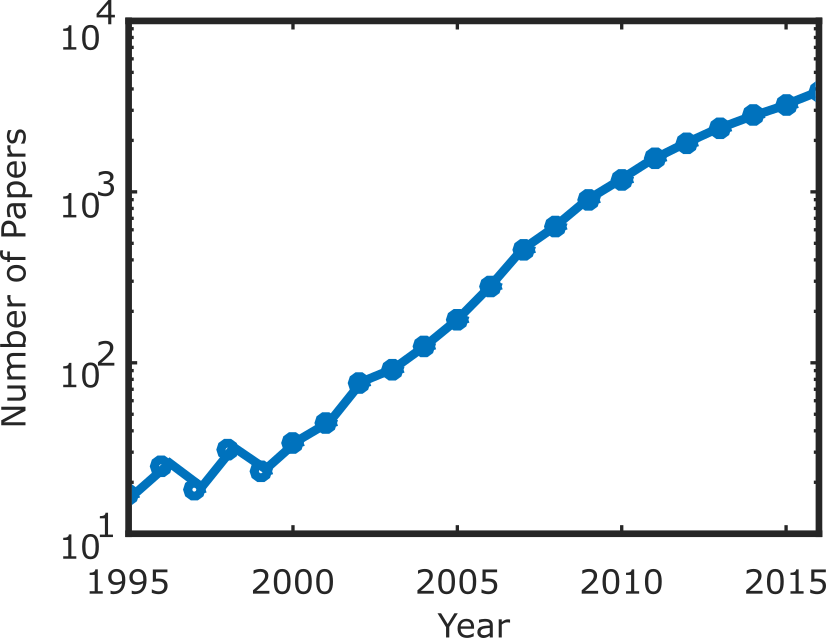
\includegraphics[width=0.40\textwidth]{Chapters/01_Introduction/Figures/paper_PT_therapy.png}
 \caption{Number of papers published containing the terms Plasmonic Photo
 Thermal Therapy since 1995. Note the logarithmic scale in the y-axis.}
 \label{fig:PPTT}
\end{figure}

During the past two decades there has been an increasing interest in gold
nanoparticles as possible agents for medical treatments. The strong interaction
between the particles and light makes them ideal candidates not only for
labelling but also for dissipating heat into very localized environments. This
simple approach can be used for instance to induce death of cancer cells and is
sometimes referred to as Plasmonic Photo Thermal Therapy (PPTT). Figure
\ref{fig:PPTT} shows the number of papers published in this field since $1995$.
The more-than-exponential increase serves as a measure for the relevance this
group of techniques is gaining. 

After decades of research there is however almost no information regarding the
exact temperature that needs to be reached by the nanoparticles to induce cell
death. Much less is available at a single-particle/single-cell level. Moreover
the field of thermometry at the nanoscale is subject to a moderate debate since
some experimental findings contradict expected values from thermodynamic
considerations. 

Chapter \ref{ch:AntiStokes} of this thesis focus into the characterization of
the mechanisms that give raise to anti-Stokes luminescence. Discarding
multi-photon processes, the only way in which is possible to observe a photon
with a higher energy than the excitation energy is through interactions with
thermal baths. In a nanoparticle electron and holes can interact amongst other
things with phonons as summarized section \ref{sec:luminescence}. 

By carefully fitting the luminescence spectra of single gold nanorods and
nanospheres it is possible to compute the surface temperature. The method
presented in chapter \ref{ch:AntiStokes} does not depend on any previous
calibration and can be performed in any confocal microscope with a couples
spectrometer. The chapter shows the increase in temperature with increasing
laser powers and also shows that the luminescence spectra changes when
increasing the medium's temperature. 

The results from the chapter can have a significant impact on an emerging
community that addresses one of the most pressing health issues nowadays. 

\subsection{Plasmon damping as function of temperature}
Luminescence is not the only way of detecting gold nanorods with an optical
microscope. Gold nanoparticles have a big scattering cross section coinciding
with the plasmon resonance. If excited with a white light source it is possible
to record the scattering spectra without much inconvenience. The shape of the
resonance is affected by the surrounding conditions. For instance changes in
refractive index of the medium induce changes in the resonance position, while
different temperatures of the particles will show different plasmon damping
rates.

In principle there are four main mechanisms responsible for the damping of
the plasmons: electron-phonon coupling, electron-surface interactions,
electron-electron collisions and radiative damping. Out of those only the
coupling with phonons shows an appreciable dependence on temperature. Therefore
studying the dependence of the plasmon width with temperature can provide
another way of measuring temperature.

Chapter \ref{ch:Damping} focuses on the characterization of the plasmon
resonance of single gold nanorods at various temperatures. The plasmon width
increases linearly with temperature, as predicted from the Debye model of
phonons. Measuring the broadening of the resonance can then be related to
changes in temperature of the surrounding medium. 

Using the scattering signal benefits from the high cross section of the
particles; however the broad distribution of widths and broadening rates found
in the studies of chapter \ref{ch:Damping} does not allow to perform an absolute
temperature measurement but to measure a relative change. This is similar to
other experiments performed with quantum dots and therefore expand the toolbox
of available techniques for thermometry at the nanoscale. 

\section{One program to rule them all}
All modern laboratories rely on computer equipment to perform measurements. It
can range from integrated micro controllers that can, for example vary the
temperature of a heating plate all the way to computers analyzing data online
and taking decisions as happens in bigger multi-billion euro experiments.
However for the average experimentalist there is a big gap between what is ideal
and what is available. 

Flexible, open source programs to control experiments are hard to find in the
internet. This generates a double negative effect: researches find themselves
reinventing the wheel more often than desired. A simple home built confocal
microscope requires a dedicated computer program to run that can take months to
develop. Readily available software normally lacks the flexibility that new
research needs, limiting the creativity of researches while thinking
experiments. 

The computer program has been made open source and can be found on Github. It
has been developed for simplifying repetitive tasks as refocusing on a particle
or triggering a spectrometer. But it also evolved into a GUI for performing and
visualizing $2$D and $3$D scans, acquiring fast timetraces, monitoring an
optical tweezer and communicating with serial devices as well as over the
network. The latest developments of the software allow to define API's for easy
integration with smartphones' applications or to control several independent
setups through a network.

All the chapters of this thesis relied on a flexible computer program that
allowed to perform tasks in an automated fashion. A direct consequence of this
is an increase in the throughput of the setup with experiments running over
night, for example. It also allowed to perform experiments that wouldn't have
been possible without a computer assisted strategy. 

Chapter \ref{ch:KCN} shows results where several particles were analyzed in an
iterative way while being etched with potassium cyanide. Refocusing on the
particles by hand is too slow for processes that happen as fast as the ones
shown in the chapter. The program allowed to refocus on selected particles and
trigger a spectrometer without user interaction. 

Chapter \ref{ch:Imaging} shows the scanning capabilities of the software for
imaging purposes. Moreover the specific program for acquiring the power
dependent plots can be written in about $20$ lines of code. When varying the
temperature of the sample as in chapters \ref{ch:AntiStokes} and
\ref{ch:Damping} it is of utmost importance being able to refocus on a reference
particle to compensate for the drift of the setup.  

The software even if developed with an optical microscope in mind, can be easily
extended to other configurations. Moreover the selection of Python as the
programming language provides platform independence; it can run without
inconvenience on several Windows versions, Mac OS and Linux. Its main objective
is to provide a lower level layer on which to build creative solutions to
complex problems.
